% begin module exponential-function-intro
\begin{frame}
\frametitle{Exponential Functions and Their Derivatives}
The function $f(x) = 2^x$ is called an exponential function because the variable $x$ is the exponent.
\uncover<2->{
\begin{definition}[Exponential Function]
In general, an exponential function is a function of the form $f(x) = a^x$, where $a$ is a positive constant.
\end{definition}
\begin{columns}[c]
\column{.3\textwidth}
\ \only<-2>{%
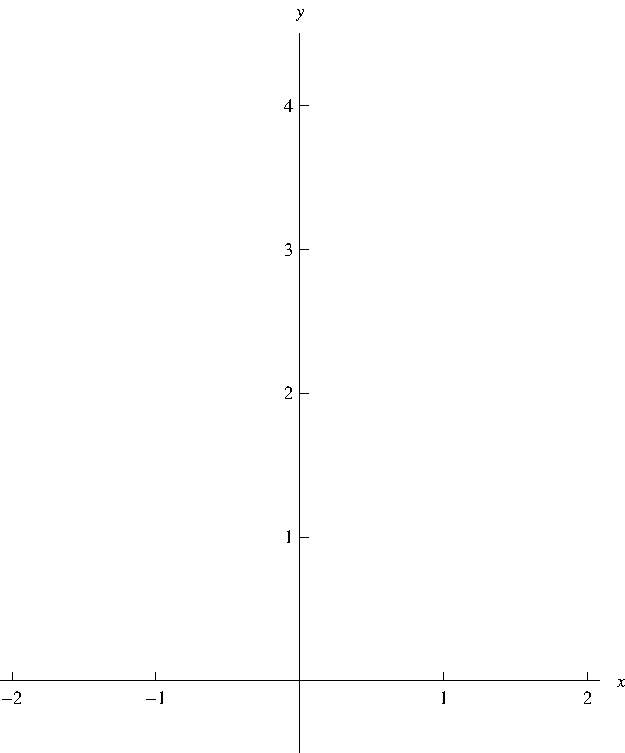
\includegraphics[height=4cm]{exponential-functions/exponential-function-intro/pictures/07-02-twoxa.pdf}%
}%
\only<3>{%
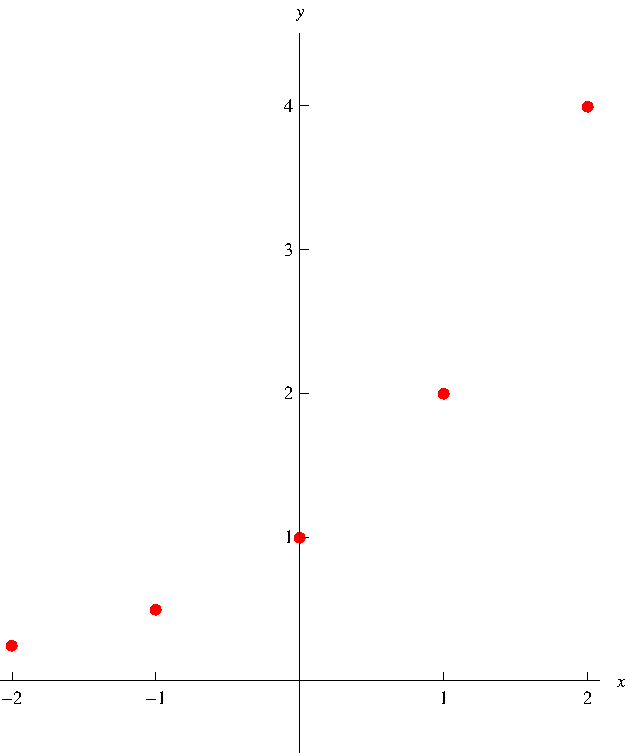
\includegraphics[height=4cm]{exponential-functions/exponential-function-intro/pictures/07-02-twoxb.pdf}%
}%
\only<4>{%
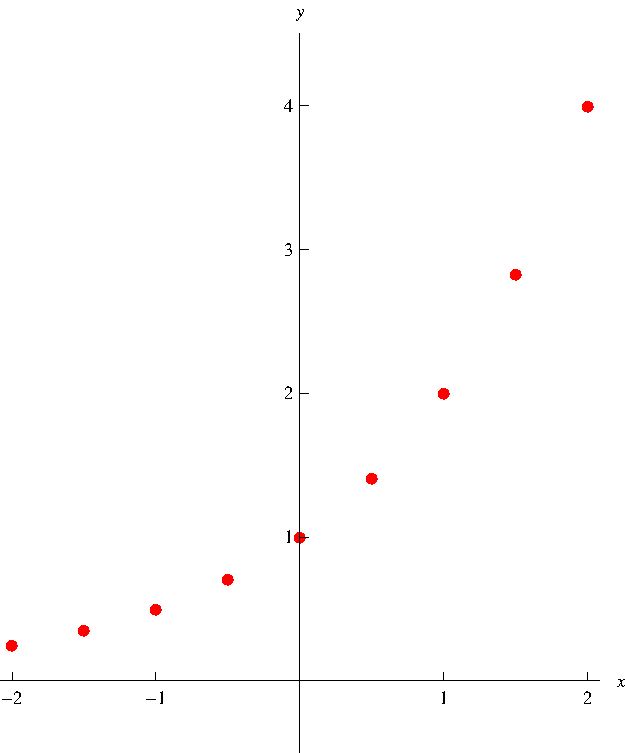
\includegraphics[height=4cm]{exponential-functions/exponential-function-intro/pictures/07-02-twoxc.pdf}%
}%
\only<5-6>{%
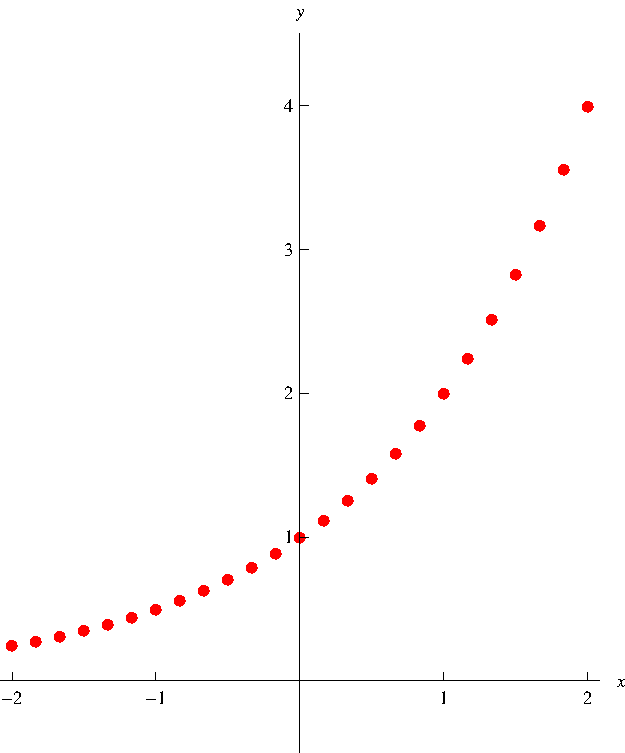
\includegraphics[height=4cm]{exponential-functions/exponential-function-intro/pictures/07-02-twoxd.pdf}%
}%
\only<7>{%
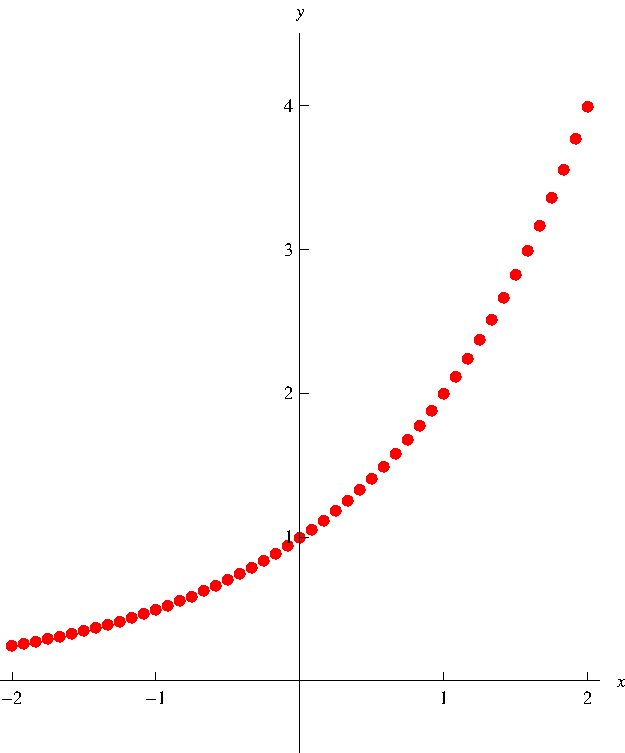
\includegraphics[height=4cm]{exponential-functions/exponential-function-intro/pictures/07-02-twoxe.pdf}%
}%
\only<8->{%
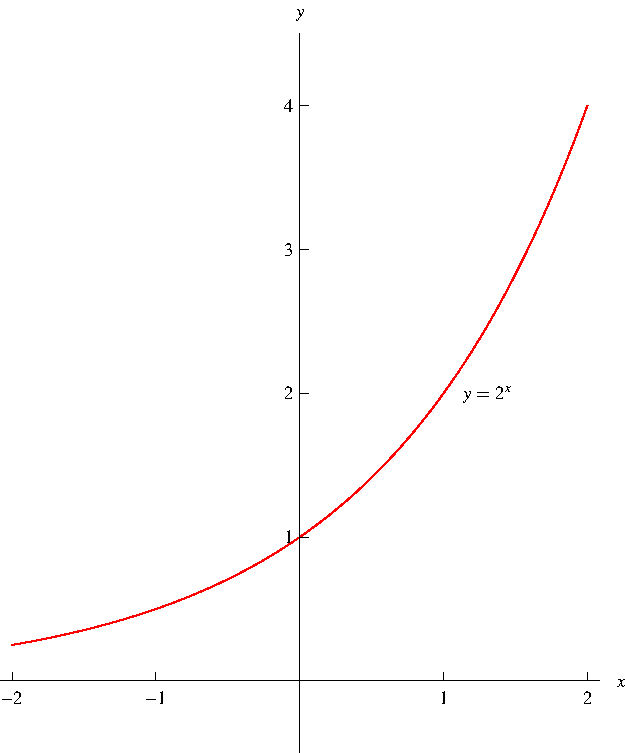
\includegraphics[height=4cm]{exponential-functions/exponential-function-intro/pictures/07-02-twoxf.pdf}%
}%
\column{.7\textwidth}
\begin{itemize}
\item<3->  $n$ a positive integer:
\item<3->  If $x = n$, then $a^n = \underbrace{a\cdot a \cdot \cdots \cdot a}_{n \textrm{ factors}}$.
\item<3->  If $x = -n$, then $a^{-n} = 1/a^n$.
\item<4->  If $x = \frac{p}{q}$ (rational), then $a^{\frac{p}{q}} = \sqrt[q]{a^p}$.
\item<6->  What if $x$ is irrational?
\item<7->  Take the limit of values at rational points: $a^x = \lim_{\frac{p}{q}\rightarrow x} a^{\frac{p}{q}}$.
\end{itemize}
}
\end{columns}
\end{frame}
% end module exponential-function-intro
